\documentclass[aspectratio=169]{beamer}

\usetheme{Madrid}
\usecolortheme{rose}

\usepackage{amsmath}
\usepackage{multirow,booktabs,setspace,caption}
\usepackage{tikz}
\usepackage{animate}
\usepackage{graphicx}

\usepackage{apacite}

%Specifying title dia
\title{Assessing Fit of IRT Models}
\author{Nina van Gerwen \& Dave Hessen}
\date{\vspace{0.5cm} \\ 14th of December, 2022 \\ \vspace{0.5cm}
\small{Methodology \& Statistics for the Behavioural, Biomedical and Social Sciences}}
\logo{
\includegraphics[width = 2 cm, height = 1 cm]{images/logo.png}}

\begin{document}

% Title dia
\maketitle

% Dia 1 -----------------------------------------------------------

% Local background:
{\usebackgroundtemplate{%
\begin{tikzpicture}[remember picture, overlay]

\node[left = 1 cm] at (current page.east){

\includegraphics[width = 8.5 cm, height = 8.5 cm]{images/roadhouse.png}

};

\end{tikzpicture}}

\begin{frame}{Outline}

\begin{enumerate}
	\item{Background information}
	\item{The issue}
	\item{The current study}
		\begin{enumerate}
			\item{Research questions}
		\end{enumerate}
	\item{Simulation study}
		\begin{enumerate}
			\item{Data generation}
			\item{Simulation design}
			\item{Performance metrics}
		\end{enumerate}
	\item{Results preview}
	\item{Questions}
	\item{References}
\end{enumerate}

\end{frame}}

%Dia 2 -----------------------------------------------------------
\begin{frame}{1. Background information}

\begin{itemize}
	\item{Item Response Theory}
		\begin{itemize}
			\item{Latent constructs}
			\item{Tests/questionnaires}
		\end{itemize}
	\item{Assessing model fit}
		\begin{itemize}
			\item{Goodness-of-fit tests}
			\item{Fit indices}
		\end{itemize}
\end{itemize}

\begin{tikzpicture}[remember picture, overlay]

\node[left = 3.5cm, below = 2 cm] at (current page.north east){


\includegraphics[width = 4 cm, height = 4 cm]{images/irt.png}

};

\end{tikzpicture}

\end{frame}

%Dia 3 -----------------------------------------------------------
\begin{frame}{2. The issue}

\begin{tikzpicture}[remember picture, overlay]

\node[below = 0.8 cm] at (current page.north){


\includegraphics[width = 8cm, height = 4 cm]{images/issue.png}

};

\end{tikzpicture}

\vspace{1cm}

\begin{itemize}
	\item{Few goodness-of-fit tests}
		\begin{itemize}
			\item{Multiple issues with current tests \footnote[frame]{\cite{chi2sens, 4plconsist1}}}
		\end{itemize}
	\item{Scarce studies for TLI\footnote[frame]{\cite{tli}} and CFI\footnote[frame]{\cite{cfi}}}
\end{itemize}

\end{frame}

%Dia 4 -----------------------------------------------------------
\begin{frame}{3. The current study}

\begin{itemize}
	\item{New goodness-of-fit test}
	\item{TLI and CFI}
\end{itemize}

\vspace{1cm}


\begin{block}{\textbf{3.1. Research questions}}

\begin{enumerate}[<+(1)->]
	\item{Required sample size?}
	\item{Comparing performance}
	\item{Performance of TLI and CFI?}
\end{enumerate}

\end{block}

\end{frame}

\begin{frame}{How will we research this?}

\begin{center}
Through a simulation study of course!


\includegraphics[width = 3.5 cm, height = 4 cm]{images/plan.png}

\end{center}

\end{frame}

%Dia 5 -----------------------------------------------------------
\begin{frame}{4. Simulation study}

\begin{block}{\textbf{4.1. Data generation}}
\begin{itemize}
	\item{Dichotomous items}
	\item{Static item parameters}
	\item{Varying four factors}
\end{itemize}

\end{block}

\end{frame}

%Dia 6 -----------------------------------------------------------
\begin{frame}{4.2. Simulation Design}

\begin{table}[htpb]
\caption{Overview of Simulation Conditions for Each Factor}
\begin{tabular}{ c c c }
\toprule
\textbf{Factor} & \textbf{Conditions} & \textbf{Description} \\
 \\
\midrule
\multicolumn{1}{l}{Test length} & 5 - 10 - 20 & \multicolumn{1}{l}{\shortstack{The total number of items that \\ the test will consist of}} \\ \\ 
\multicolumn{1}{l}{Sample size} & \shortstack{100 - 200 - 500 \\ 1000 - 1500} & \multicolumn{1}{l}{\shortstack{The total number of observations \\ that are available for each item}} \\ \\
\multicolumn{1}{l}{Model type} & 2PL - 3PL & \multicolumn{1}{l}{\shortstack{The models that we will use as \\ the basis for data generation}} \\ \\
\multicolumn{1}{l}{Number of groups} & 2 - 3 - 4 & \multicolumn{1}{l}{\shortstack{The number of groups that the data \\ gets divided into for the LR \\ Randomisation test calculations}} \\

\bottomrule
\end{tabular}

\label{tab:1}
\end{table}

\end{frame}

%Dia 7 -----------------------------------------------------------
\begin{frame}[t]{4.3. Performance metrics}

\begin{columns}

\begin{column}{0.5\textwidth}
	\begin{center}
\textbf{Goodness-of-fit tests}
	\end{center}
	
\begin{itemize}
	\item{Power}
	\item{Empirical $\alpha$}
\end{itemize}

\end{column}

\begin{column}{0.5\textwidth}
	\begin{center}
\textbf{Fit indices}
	\end{center}

\begin{itemize}
	\item{Mean (SE)}
\end{itemize}

\end{column}

\end{columns}
\vspace{1cm}

\includegraphics[width = 0.5\textwidth]{images/power.png}

\end{frame}

\begin{frame}{5. Preview of the results}

\begin{columns}

\begin{column}{0.5\textwidth}
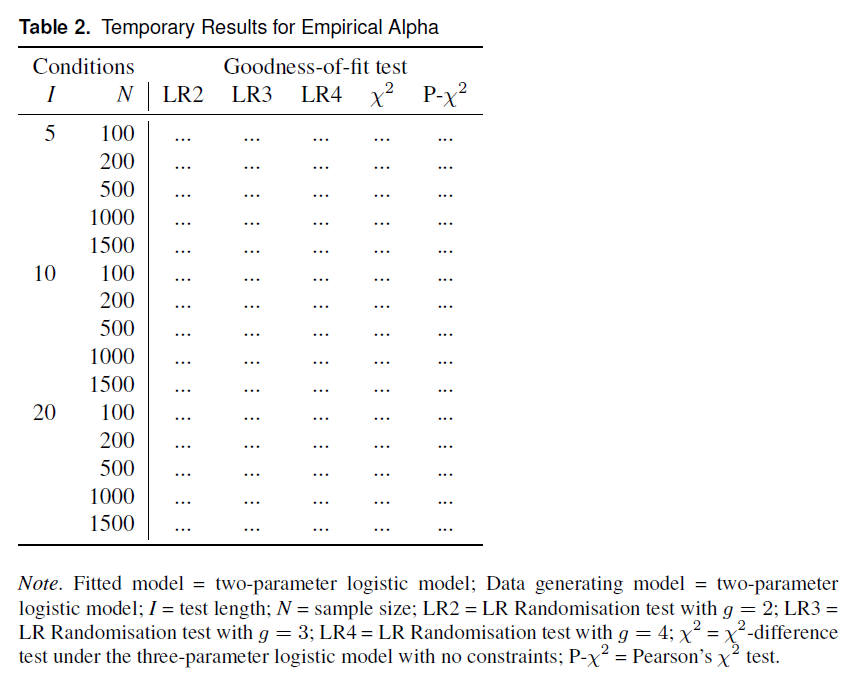
\includegraphics[width = \textwidth]{images/table2.png}
\end{column}

\begin{column}{0.5\textwidth}
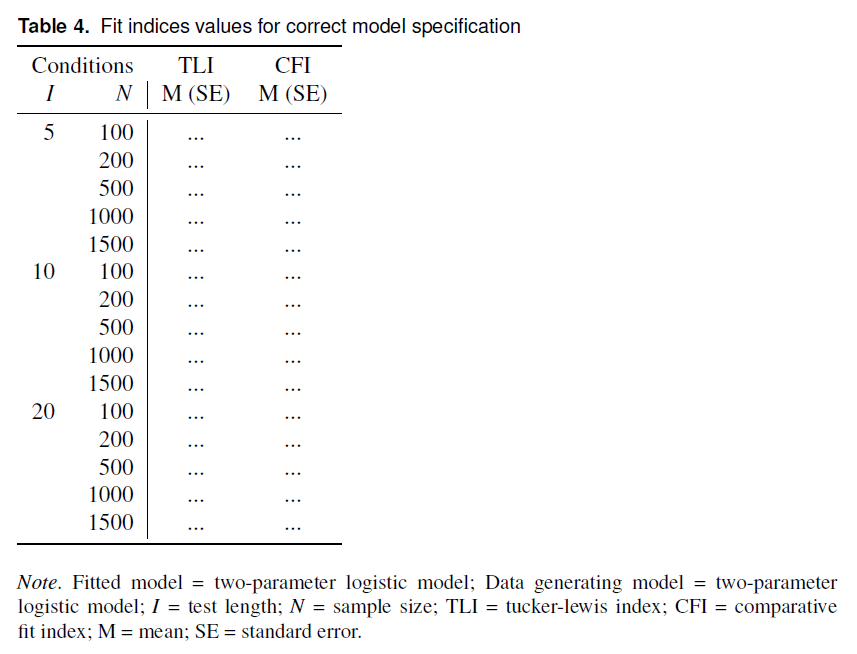
\includegraphics[width = \textwidth]{images/table3.png}
\end{column}

\end{columns}

\end{frame}

%Dia 8 -----------------------------------------------------------
\begin{frame}[c]{Thank you for listening!}

\begin{center}


\includegraphics[width=8cm, height=5cm]{images/questions.png}

\end{center}

\begin{tikzpicture}[remember picture, overlay]

\node[left = 6cm, below = 1 cm] at (current page.east){

\animategraphics[loop, width = 3cm]{7}{images/corgif-}{0}{5}

};

\end{tikzpicture}


\end{frame}

%Dia 9 -----------------------------------------------------------
\begin{frame}{References}
\bibliographystyle{apacite}
\bibliography{reportref}

\end{frame}

\end{document}